
\chapter{Performing operations over polytopes}
\label{ch:operations_over_poly_stategies}

Once the polytopes are transformed in standard forms such as $\repr{H}$ or $\repr{V}$-representations, they can be exploited to efficiently calculate different operations over multiple polytopes, such as Minkowski sums  and intersections.

\section{Minkowski sum of polytopes}
\begin{figure}[!h]
    \centering
    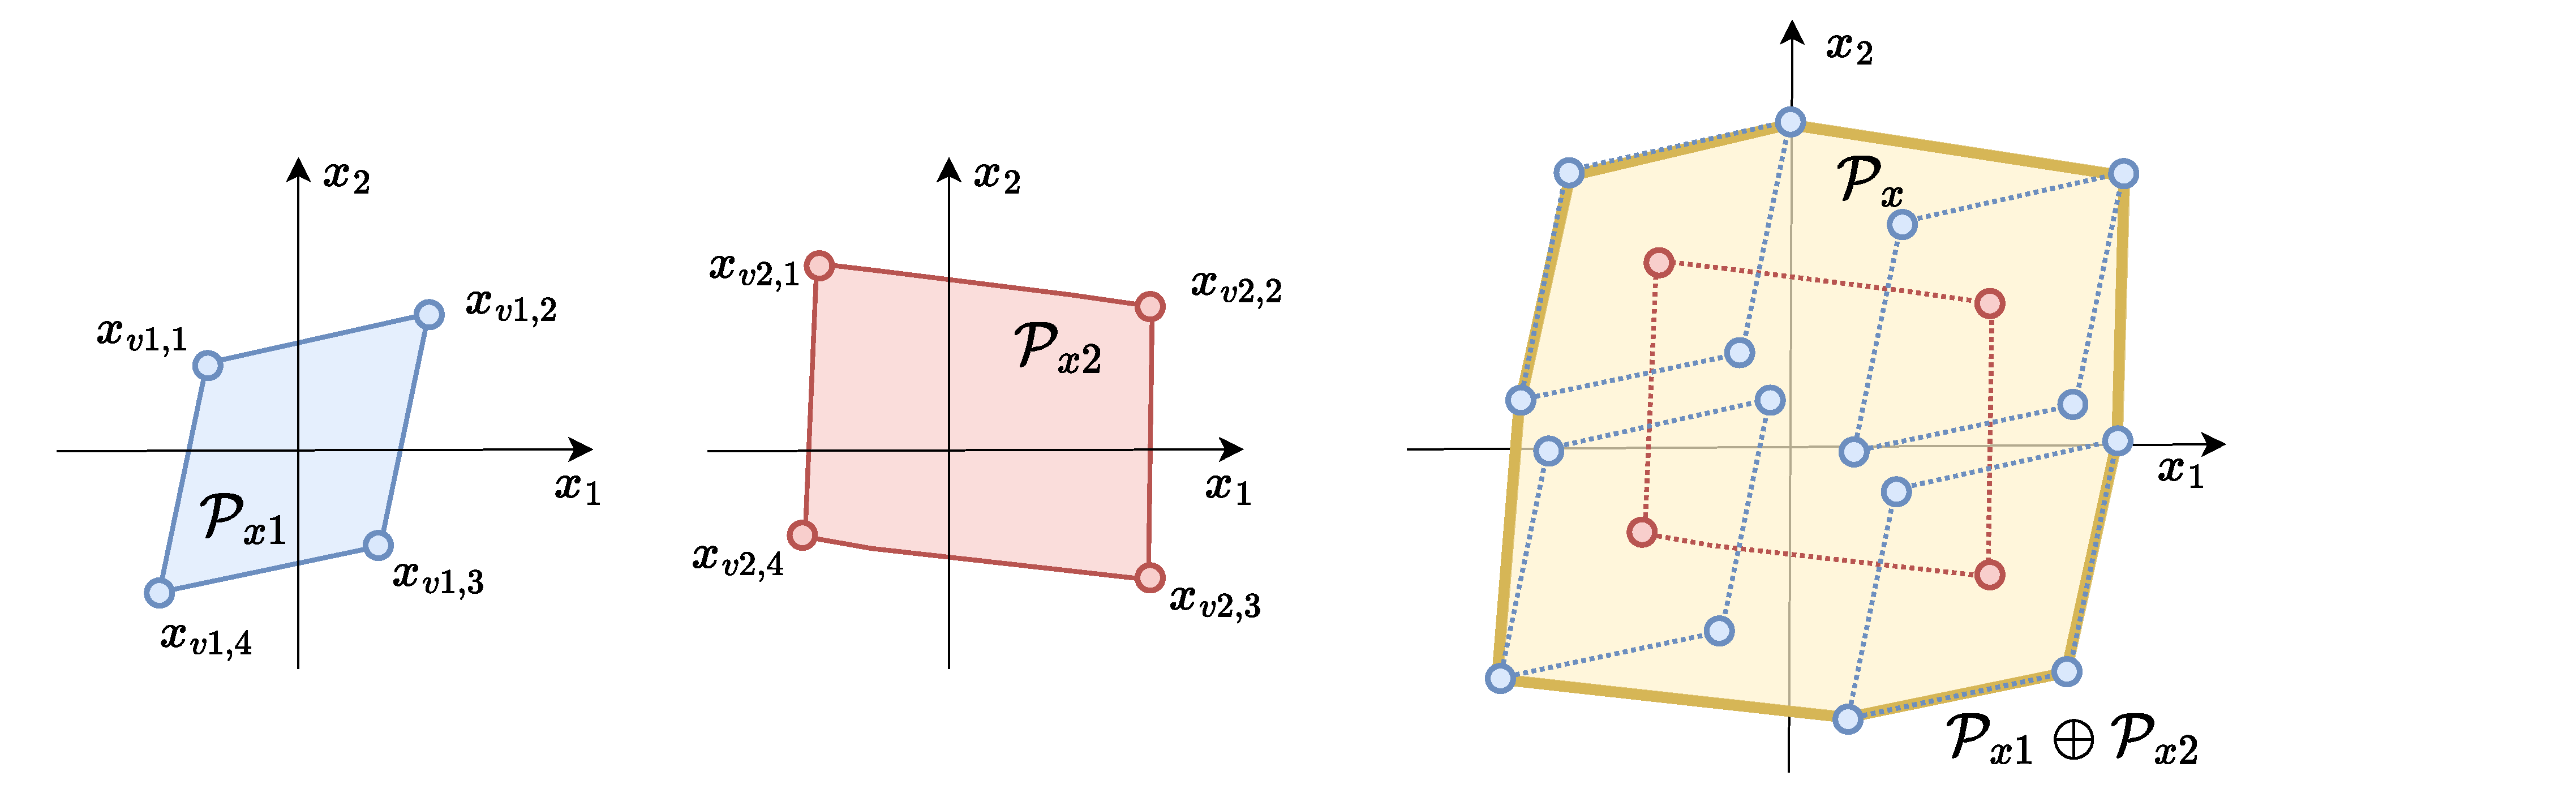
\includegraphics[width=0.9\linewidth]{Chapters/imgs/polytope_minkowski_sum.pdf}
    \caption{A 2d ($m\!=\!2$) example of the construction of the intersection of two polytopes using their $\repr{V}$-representation. The points representing the vertices of the polytope $\mathcal{P}_{x1}$ are shown in blue, and for polytope $\mathcal{P}_{x2}$ in red. The Minkowski sum polytope $\mathcal{P}_x$ is formed by calculating all the combinations of all the vertices of both polytopes, and then calculating their convex hull, the hull is shown in yellow color.}
    \label{fig:collab_sum_solution}
\end{figure}

In order to calculate Minkowski sum of multiple polytopes, for example two polytopes $\mathcal{P}_{x1}$ and $ \mathcal{P}_{x2}$
\begin{equation}
    \mathcal{P}_x = \mathcal{P}_{x1} \oplus \mathcal{P}_{x2}
\end{equation}
the most straight-forward approach is to express both polytopes in their $\repr{V}$-representation form
\begin{equation}
    \mathcal{P}_{x1} = \conv{\bm{x}_{v1,1},~\bm{x}_{v1,2},~\ldots~,\bm{x}_{v1,N_1}}
\end{equation}
\begin{equation}
    \mathcal{P}_{x2} =  \conv{\bm{x}_{v2,1},~\bm{x}_{v2, 2},~\ldots~,\bm{x}_{v2,N_2}}
\end{equation}
where polytope $\mathcal{P}_{x1}$ has $N_1$ vertices $\bm{x}_{v1,i}\in \mathbb{R}^m$, and polytope $\mathcal{P}_{x2}$ has $N_2$ vertices $\bm{x}_{v2,i}\in \mathbb{R}^m$.

Then the Minkowski sum of the polytopes can be found as the convex-hull of all the $N_1\!\cdot\!N_2$ combinations of all the vertices of the two polytopes
\begin{equation}
\begin{split}
    \mathcal{P}_x =  conv\big\{&\bm{x}_{v1,1} + \bm{x}_{v2,1},~ \ldots~,\bm{x}_{v1, N_1} + \bm{x}_{v2,1},\\&\bm{x}_{v1,1} + \bm{x}_{v2,2},~\ldots~,\bm{x}_{v1, N_1} + \bm{x}_{v2,2},\\&~\ldots~\\
    &\bm{x}_{v1, 1}  +\bm{x}_{v2,N_2}, ~\ldots~ ,\bm{x}_{v1, N_1} +\bm{x}_{v2,N_2}\big\}
\end{split}
\end{equation}
These $N_1\!\cdot\!N_2$ are not all vertices of the polytope $\mathcal{P}_x$, some of them are inside of the polytope, as shown on a graphical example of the Minkowski sum of two  2d ($m=2$) polytopes on Figure \ref{fig:collab_sum_solution}. In order to find the minimal set of vertices of the polytope $\mathcal
{P}_x$, defining its $\repr{V}$-representation, different convex-hull algorithms \cite{Barber1996} can be used.

Once the $\repr{V}$-representation is determined, different standard representation conversion algorithms (section \ref{ch:standard_represtantion_conversion}), can be used to efficiently find its $\repr{H}$-representation.


\subsection{Special case - projection formulation}
A special case of simplified Minkowski sum calculation arises when polytopes $\mathcal{P}_{x1}$ and $\mathcal{P}_{x2}$ both have projection formulation
\begin{equation}
    \mathcal{P}_{x1}=\{\bm{x}_1\in\mathbb{R}^m |~ \bm{x}_1 = B_1\bm{y}_1,~\bm{y}_1 \in \mathcal{I}_1  \}
\end{equation}
\begin{equation}
    \mathcal{P}_{x2}=\{\bm{x}_2\in\mathbb{R}^m |~ \bm{x}_2 = B_2\bm{y}_2,~\bm{y}_2 \in \mathcal{I}_2  \}
\end{equation}
where both polytopes are defined in the comon $m$ dimensional output space $\bm{x}_1,\bm{x}_2\in\mathbb{R}^m$, while their input spaces $\bm{y}_1\in\mathbb{R}^{n_1}$,$\bm{y}_2\in\mathbb{R}^{n_2}$ might have different dimensions $n_1\neq n_2$ and are limited, in generic case, by polytope input sets $\mathcal{I}_1$ and $\mathcal{I}_2$.
\begin{equation}
    \mathcal{I}_{1}=\{\bm{y}_1\in\mathbb{R}^{n_1} ~|~ H_1\bm{y}_1 \leq \bm{d}_1\}, \qquad
    \mathcal{I}_{2}=\{\bm{y}_2\in\mathbb{R}^{n_2} ~|~ H_2\bm{y}_2 \leq \bm{d}_2\}
\end{equation}

As the Minkowski sum of two polytopes can then be expressed as the achievable set of output variable $\bm{x}\in\mathbb{R}^m$ corresponding the sum of the variables $\bm{x}_1$ and $\bm{x}_2$
\begin{equation}
    \mathcal{P}_{x}= \mathcal{P}_{x1} \oplus \mathcal{P}_{x2} = \{\bm{x}\in\mathbb{R}^m ~|~ \bm{x} =  \bm{x}_1 + \bm{x}_2, \quad \bm{x}_1 \in \mathcal{P}_{x1}, ~\bm{x}_2 \in \mathcal{P}_{x2},  \}
\end{equation}
the projection formulation of their Minkowski sum can be expressed directly
\begin{equation}
    \mathcal{P}_{x}=\left\{\bm{x}\in\mathbb{R}^m ~\bigg|~ 
    \bm{x} = \begin{bmatrix}
        B_1 & 0 \\
        0 & B_2
    \end{bmatrix}\begin{bmatrix}
        \bm{y}_1 \\
        \bm{y}_2
    \end{bmatrix}, ~\begin{bmatrix}
        H_1  \\
        H_2
    \end{bmatrix} \begin{bmatrix}
        \bm{y}_1 \\
        \bm{y}_2
    \end{bmatrix} \leq \begin{bmatrix}
        \bm{d}_1  \\
        \bm{d}_2
    \end{bmatrix} \right\}
\end{equation}

Finding the $\repr{V}$ and $\repr{H}$-representation of this polytope can then be done using the approaches  for polytope with projection formulation, described in chapter \ref{ch:projection_algos}.

\paragraph*{} The same logic can be used if the Minkowski sum is calculated for more than two polytopes 
\begin{equation}
    \mathcal{P}_x = \mathcal{P}_{x1} \oplus \mathcal{P}_{x2} \oplus ~\cdots
\end{equation}

\section{Polytope intersection}

\begin{figure}[!h]
    \centering
    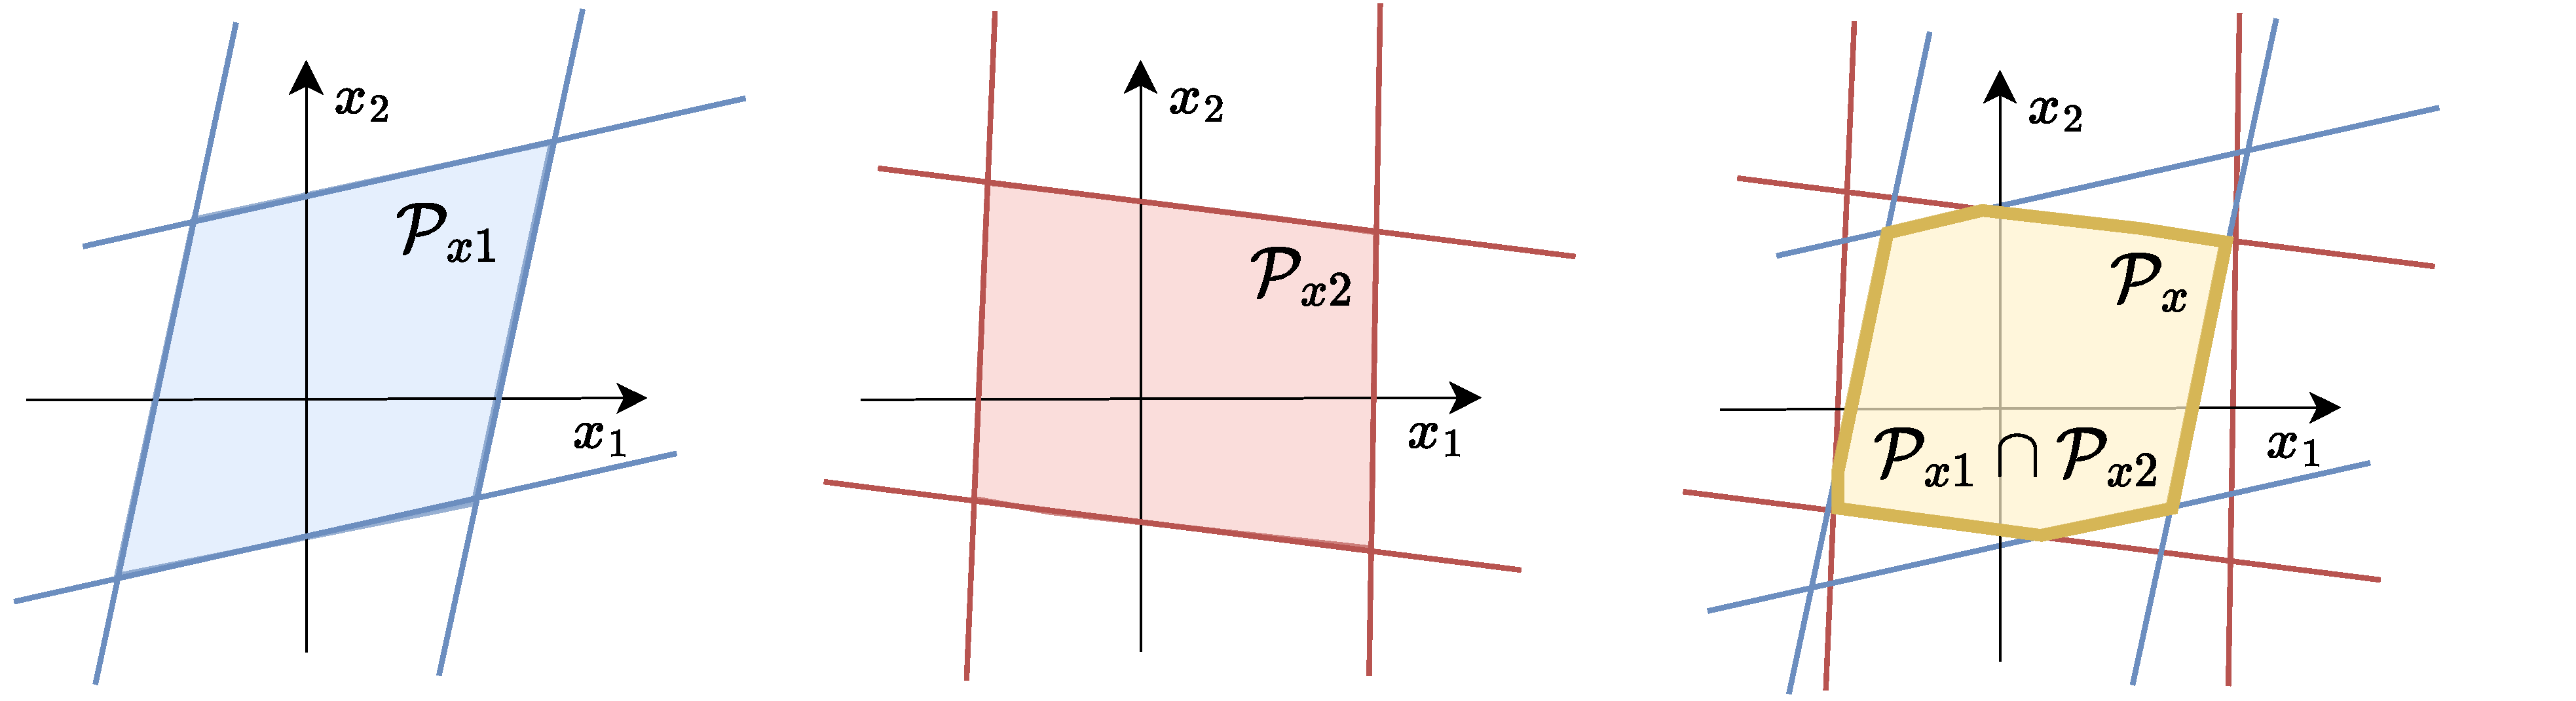
\includegraphics[width=0.8\linewidth]{Chapters/imgs/polytope_intersection.pdf}
    \caption{A 2d ($m\!=\!2$) example of the construction of the intersection of two polytopes using their $\repr{H}$-representation. The lines representing half-planes of the polytope $\mathcal{P}_{x1}$ are shown in blue, and for polytope $\mathcal{P}_{x2}$ in red. The intersection polytope $\mathcal{P}_x$ is formed by including all of their half-planes, where the space representing their intersection is shown in yellow.}
    \label{fig:collab_intesection_solution}
\end{figure}

In order to calculate an intersection of multiple polytopes, for example two polytopes $\mathcal{P}_{x1}$ and $ \mathcal{P}_{x2}$
\begin{equation}
    \mathcal{P}_x = \mathcal{P}_{x1} \cap \mathcal{P}_{x2}
\end{equation}
the simplest approach is to transform both polytopes to their $\repr{H}$-representation
\begin{equation}
    \mathcal{P}_{x1} = \{\bm{x}\in\mathbb{R}^m ~|~ H_1\bm{x}\leq \bm{d}_1\}
\end{equation}
\begin{equation}
    \mathcal{P}_{x2} = \{\bm{x}\in\mathbb{R}^m ~|~ H_2\bm{x}\leq \bm{d}_2\}
\end{equation}
where polytopes $\mathcal{P}_{x1}$ and  $\mathcal{P}_{x2}$ represent limits of the same output variable $\bm{x}\in\mathbb{R}^m$. Additionally matrices $H_i\in\mathbb{R}^{m\times N_i}$ and vectors $\bm{d}_i\in\mathbb{R}^{N_i}$ define the half-plane representation of the polytopes $\mathcal{P}_{xi}$ with $N_i$ faces.

Given their $\repr{H}$-representations the intersections of these polytopes can be expressed directly as
\begin{equation}
    \mathcal{P}_x = \left\{\bm{x}\in\mathbb{R}^m ~\bigg|~ \begin{bmatrix}
        H_1\\
        H_2
    \end{bmatrix}\bm{x}\leq \begin{bmatrix}
        \bm{d}_1\\
        \bm{d}_2
    \end{bmatrix}\right\}
\end{equation}
by stacking their matrices $H_i$ and vectors $\bm{d}_i$ forming the $\repr{H}$-representation of the polytope $\mathcal{P}_x$. The obtained $\repr{H}$-representation might not be minimal though, it might have some redundant inequalities. If the application requires it, they can be removed using standard algorithms \cite{Paulraj2006}.
A visual example of constructing the intersection of $m=2$ dimensional polytopes using their $\repr{H}$-representation is shown on Figure \ref{fig:collab_intesection_solution}.

Once the $\repr{H}$-representation is determined, different standard representation conversion algorithms (section \ref{ch:standard_represtantion_conversion}), can be used to efficiently find its $\repr{V}$-representation.

\subsection{Special case - intersection formulation}

A special case of simplified polytope intersection calculation arises when polytopes $\mathcal{P}_{x1}$ and $\mathcal{P}_{x2}$ both have intersection formulation
\begin{equation}
    \mathcal{P}_{x1}=\{\bm{x}\in\mathbb{R}^m |~ A_1\bm{x} = \bm{y}_1,~\bm{y}_1 \in \mathcal{I}_1  \}
\end{equation}
\begin{equation}
    \mathcal{P}_{x2}=\{\bm{x}\in\mathbb{R}^m |~ A_2\bm{x} = \bm{y}_2,~\bm{y}_2 \in \mathcal{I}_2  \}
\end{equation}
where both polytopes are defined in the common $m$ dimensional output space $\bm{x}\in\mathbb{R}^m$, while their input spaces $\bm{y}_1\in\mathbb{R}^{n_1}$,$\bm{y}_2\in\mathbb{R}^{n_2}$ might have different dimensions $n_1\neq n_2$ and are limited, in generic case, by polytope input sets $\mathcal{I}_1$ and $\mathcal{I}_2$.
\begin{equation}
    \mathcal{I}_{1}=\{\bm{y}_1\in\mathbb{R}^{n_1} ~|~ H_1\bm{y}_1 \leq \bm{d}_1\}, \qquad
    \mathcal{I}_{2}=\{\bm{y}_2\in\mathbb{R}^{n_2} ~|~ H_2\bm{y}_2 \leq \bm{d}_2\}
\end{equation}

Using these polytope formulations their intersection polytope can be expressed in the intersection formulation by stacking the equations
\begin{equation}
    \mathcal{P}_{x}=\left\{\bm{x}\in\mathbb{R}^m ~\bigg|~ 
   \begin{bmatrix}
        A_1 \\
        A_2
    \end{bmatrix} \bm{x} = \begin{bmatrix}
        \bm{y}_1 \\
        \bm{y}_2
    \end{bmatrix}, ~\begin{bmatrix}
        H_1  \\
        H_2
    \end{bmatrix} \begin{bmatrix}
        \bm{y}_1 \\
        \bm{y}_2
    \end{bmatrix} \leq \begin{bmatrix}
        \bm{d}_1  \\
        \bm{d}_2
    \end{bmatrix} \right\}
\end{equation}


Finding the $\repr{V}$ and $\repr{H}$-representation of this polytope can then be done using the approaches for polytope with intersection formulation, described in chapter \ref{ch:intersection_algos}.


\paragraph*{} The same logic can be used if the intersection is calculated for more than two polytopes 
\begin{equation}
    \mathcal{P}_x = \mathcal{P}_{x1} \cap \mathcal{P}_{x2} \cap ~\cdots
\end{equation}
